\newpage\section{Introduction} \label{sec:intro}
Here is an example of a description, a semi-customized way to do a labeled itemized list of described items.

\begin{description}
    \item[Line label] Your description
    \item[Goose] A beautiful bird
\end{description}

\noindent
And here is an equation that's aligned along the equal sign by using split:

\begin{equation} \label{eq:example}
\begin{split}
    \lambda_G(\nabla_G, a, b, c) & = c_a + b \\
    \nabla_G & = a^b - c
\end{split}
\end{equation}
\noindent
Good luck. You can refer to equations too much like sections. For instance, look at my~\autoref{eq:example}. Oh and here's a citation example~\cite{Goodfellow2014GenerativeNetworks}.

Here is an example of a~\autoref{fig:cat}:

\begin{figure}[H] \centering % H to force position, or [tbh] for more loose placement (recommended)

    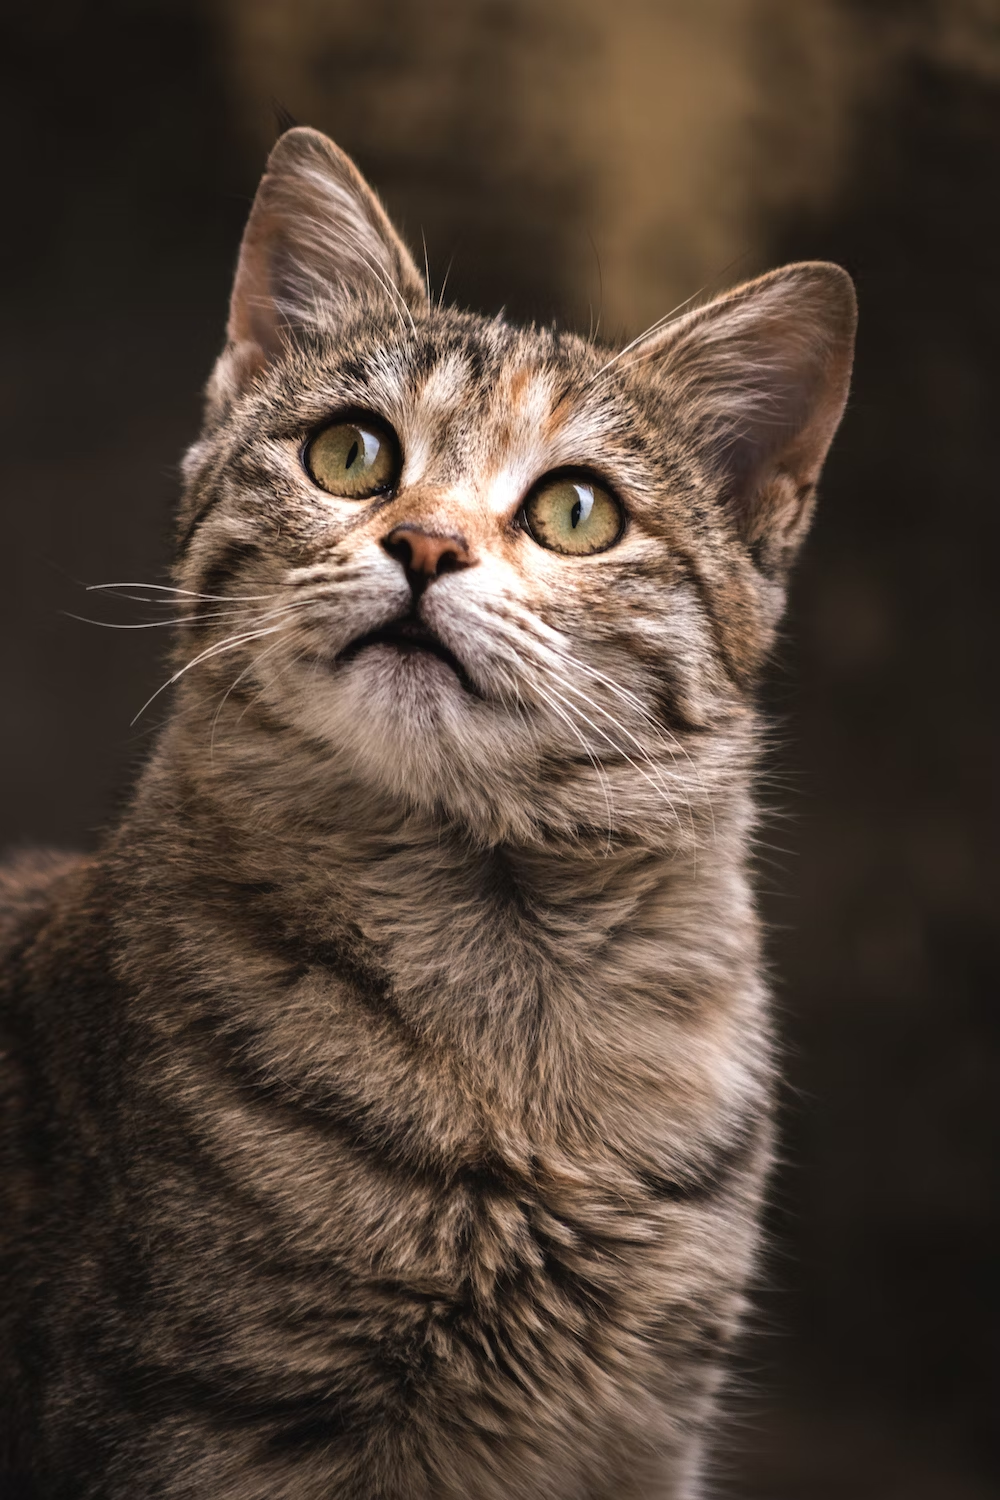
\includegraphics[width=0.5\textwidth]{figures/cat.png}

    \caption{A cool cat.}

    \label{fig:cat}

\end{figure}

\section{Analysis}
\lipsum[]

\subsection{Specific analysis}
\lipsum[]

\subsubsection{Even more specific}
\lipsum[]

\myparagraph{(Doesn't appear in TOC) Extra specific}
\lipsum[]

\newpage
\mysubparagraph{(Not in TOC) Unnumbered extra notes}
You can refer to labels automatically, check out~\autoref{sec:intro} for example of a description list.